\chapter{Stand der Forschung}
\label{StandDerForschung}

Die Idee eines Homomorphen Kryptosystems entstand bereits 1978 \cite{Rivest1978ONDB}, jedoch war lange nicht klar, ob solch eine voll homomorphe Verschlüsselung (Full Homomophe Encryption - FHE) möglich ist. Im Jahr 2009 entwickelte Craig Gentry solch ein FHE-Schema, welches eine beliebige Anzahl an Addition und Multiplikation durchführen kann \cite{Gentry2009AFH}. 

\begin{figure}
  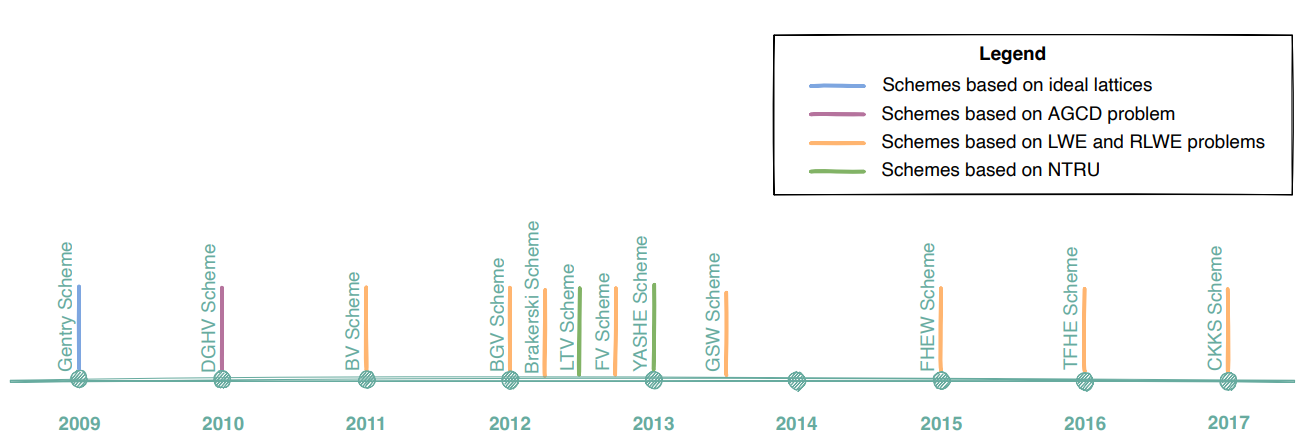
\includegraphics[scale=0.45]{bilder/FHE-Timeline.png}
  \caption{FHE Zeitlinie \cite{FHESurvey}}
  \label{fig:FheTimeline}
\end{figure}

Danach folgten mehrere Versuche dieses System zu verbessern, wie das 2011 erschiene BGV schema \cite{BGV} und das 2012 erschiene FV schema \cite{FV}. Beide Systeme sind LWE/RLWE basiert und unterscheiden sich im wesentlichen in der art und weise, wie sie mit dem wachsenden Fehler, vor allem bei der Multiplikation umgehen und diesen wieder reduzieren. Es folgten weitere Entwicklungen (siehe \ref{fig:FheTimeline}), aber auch Schwachstellen, wie die 2020 entdeckten Schwachstellen für CKKS \cite{SecurtyCKKS}.

Neben der Entwicklung neuer FHE-Schemas wurden auch versucht die bereits verfügbaren effizient zu Implementieren  \cite{FheImplementations}. Jedoch sind alle bisherigen FHE-Schemas schon von sich aus sehr ineffizient, wodurch es kaum praktische Einsätze dieser gibt.

Um dieses Problem zu lösen wird auch schon länger daran geforscht, FHE-Schemas direkt in Hardware umzusetzen und somit effizienter laufen zu lassen \cite{FheHardware2014} \cite{FheHardware2023}. 
